\chapter{Diseño}\label{chap:diseno}

\section{Proyecto como servicio}
Un proyecto como servicio es una aplicación modular y distribuida en la que el backend funciona como un servicio independiente de la plataforma, permitiendo la interacción con varios tipos de clientes (web, móvil, etc.) con conexión a Internet. 

Presenta gran flexibilidad ante la impementación de mejoras, ya que se pueden realizar cambios en el backend sin afectar al frontend, y viceversa. Como puede ser agregar nuevas funcionalidades o módulos (como más servicios de análisis de gastos o incorporar diferentes funcionalidades de ahorro) sin afectar el resto del sistema. A medida que los usuarios crecen, el backend como servicio puede escalarse fácilmente. De esta manera, se adapta bien a un entorno donde puede servir como base para otros clientes o dispositivos, es un sistema versátil y eficiente. Sin embargo, también presenta desventajas, como dependencia de la red, ya que requiere conexión entre cliente y servidor, lo cual puede ser una limitación si el servicio se utiliza sin darse esa condición\cite{galster2014variability}.

Este proyecto sigue un enfoque como servicio, ya que se espera que la aplicación pueda ser utilizada por un número creciente de usuarios y que se puedan implementar mejoras frecuentes y nuevas funcionalidades en el futuro, motivado principalmente por el uso de metodología ágil en el desarollo de la misma. Además es importante que se disponga de acceso multiplataforma, puesto que desarrollarán funcionalidades útiles para dispositivos móviles (como el uso del GPS) y otras más orientadas a su uso en ordenador (como las consultas detalladas de los movimientos realizados por el usuario, donde se obtendrá mayor comodidad para analizar el potencial volúmen de datos). En mayo de 2024, un estudio de la CNMC\footnote{Comisión Nacional de los Mercados y la Competencia} reveló que el 80\% de las personas en España acceden diariamente a Internet, por ello se considera que la mayoría de los usuarios de la aplicación tendrán acceso a la red y podrán utilizarla sin problemas\cite{cnmc2024}. 
De este modo, se determina la creación de una una aplicación web.

\begin{figure}[ht!]
    \centering
    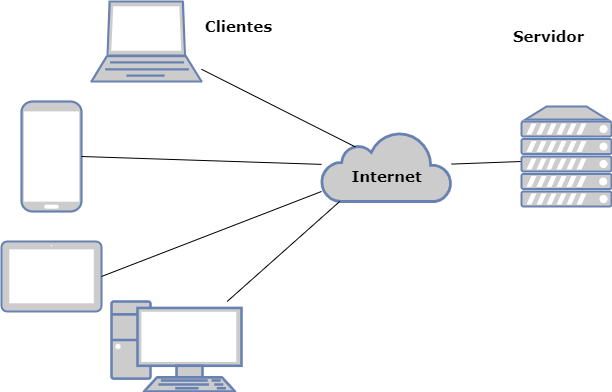
\includegraphics[height = 50mm]{imagenes/proyecto_servicio.drawio.png}
    \caption{Proyecto como servicio}
    \label{fig:proyecto_como_servicio}
\end{figure}


\section{Arquitectura software}
La arquitectura software de un proyecto podría definirse como la estructura y organización de los elementos que lo componen, así como las relaciones y dependencias entre ellos. Es un aspecto importante en el diseño de una aplicación, ya que permite orientarla hacia el logro de los objetivos planteados y tiene en consideración la posible evolución del sistema: su comprensión, escalabilidad, mantenimiento y rendimiento\cite{fernandez2006arquitectura}.
Para definir la arquitectura de software de la aplicación, se analizaron varias opciones disponibles, cada una con características y beneficios diferentes\cite{albin2003art}\cite{garimilla2024art}:

\begin{itemize}
\item Arquitectura Monolítica\\
Las arquitecturas monolíticas agrupan todos los componentes de la aplicación en una única unidad de despliegue, lo cual facilita la implementación y es adecuado para aplicaciones pequeñas o medianas. Sin embargo, este enfoque suele presentar limitaciones en cuanto a flexibilidad y escalabilidad, ya que todos los módulos están estrechamente acoplados. Lo que provoca que las opciones de actualización y expansión se vean reducidas.

\item Arquitectura Basada en Microservicios\\
Una arquitectura de microservicios organiza la aplicación en servicios pequeños e independientes que pueden desarrollarse, desplegarse y escalarse de manera autónoma. Cada microservicio puede implementarse con el lenguaje y las herramientas más adecuadas para su función, lo que aporta flexibilidad y facilita la escalabilidad. Además, su naturaleza distribuida añade seguridad, ya que los servicios se comunican a través de una API y no de manera directa, ofreciendo una capa adicional de protección. Sin embargo, esta estructura aumenta la complejidad de implementación y requiere mayor infraestructura, lo cual puede ser innecesario para aplicaciones como esta con un alcance más específico\cite{RedHat2023}\cite{lopez2017arquitectura}.

\item Arquitectura Cliente-Servidor\\
La arquitectura cliente-servidor divide la aplicación en dos componentes principales: el cliente (interfaz de usuario) y el servidor (lógica de negocio y acceso a datos). La comunicación entre cliente y servidor se puede gestionar mediante una API REST (Representational State Transfer), que utiliza solicitudes HTTP\footnote{HyperText Transfer Protocol: es un protocolo cliente-servidor para comunicar aplicaciones por medio de peticiones de datos y recursos.} (como GET, POST, PUT y DELETE) para intercambiar información. Este enfoque proporciona una separación clara entre la interfaz y la lógica de negocio, facilitando el mantenimiento y la escalabilidad sin necesidad de una infraestructura compleja como en el caso de los microservicios.

\end{itemize}

Los enfoques tradicionales con arquitectura monolítica limitan a los desarrolladores en cuanto al lenguaje de programación y entorno de ejecución. Por otro lado, las otras dos opciones permiten a los desarrolladores elegir el lenguaje de programación y el entorno de ejecución más adecuado para cada servicio. Además, por su naturaleza distribuida facilitan la escalabilidad y la flexibilidad del sistema, y aportan seguridad al actuar como una primera línea de defensa ante ataques, ya que los servicios se comunican entre sí por ejemplo mediante una API y no directamente. 

La arquitectura basada en microservicios no se justifica para las necesidades actuales del proyecto, que al resolver una necesidad específica no se beneficia de las ventajas que ofrece pero si podría verse afectado su desarrollo por la complejidad que añade. 

En su lugar, se ha optado por implementar una arquitectura cliente-servidor para la aplicación, donde el cliente (generalmente un navegador web) se corresponde con la interfaz de usuario y el servidor gestiona la lógica de negocio y la base de datos. La comunicación entre ambos se realiza mediante una API REST. Esto permite modularidad, escalabilidad, y facilidad de mantenimiento, facilitando una futura migración a microservicios si es necesario, ya que la API REST puede servir como interfaz entre servicios independientes. La API REST en esta arquitectura conecta de forma sencilla y eficiente los datos y funcionalidades del backend con el frontend, pensada como una colección de herramientas escalable e independiente que realizan tareas específicas. 

\section{Diseño lógico}

\subsection{Diagrama de clases}
Diagramas UML? (clases, secuencia...)

\subsection{Diagrama Entidad-Relación}
El diagrama entidad-relación es una representación gráfica de las entidades y las relaciones entre ellas en una base de datos. Permite visualizar la estructura de la base de datos y las restricciones que se aplican a los datos. En el caso de la aplicación, se ha diseñado para representar las entidades principales y las relaciones entre ellas, con el objetivo de definir la estructura de la base de datos para facilitar su implementación (Figura \ref{fig:diagrama_ER}).

\begin{figure}[ht!]
    \centering
    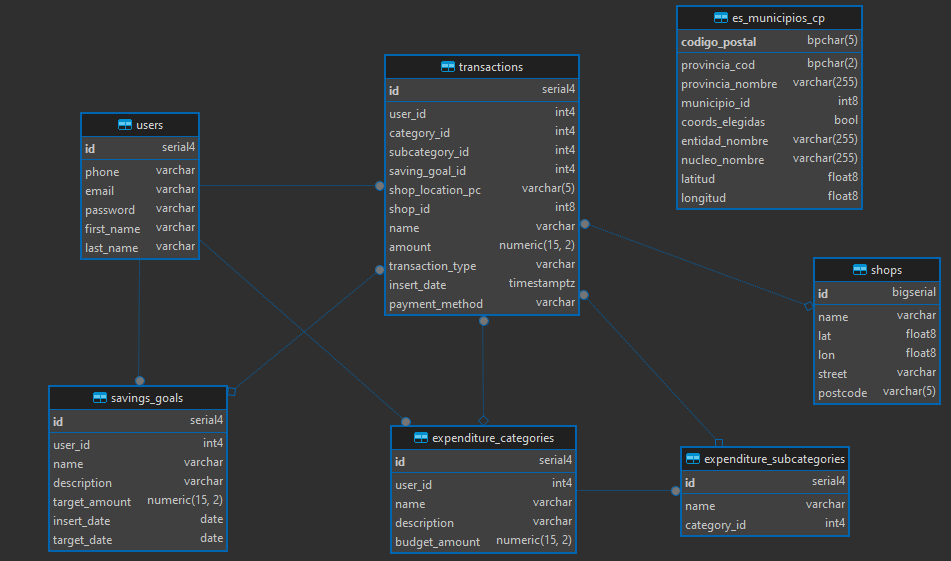
\includegraphics[height=50mm]{imagenes/diagrama_ER.png}
    \caption{Diagrama Entidad-Relación de la capa de datos}
    \label{fig:diagrama_ER}
\end{figure}


\section{Diseño interfaz de usuario y navegación en la plataforma}
\label{sec:diseno_interfaz_usuario}
La interfaz de usuario es un aspecto fundamental en el diseño de una aplicación, ya que es la primera impresión que recibe el usuario y determina en gran medida su experiencia de uso. Una interfaz bien diseñada debe facilitar la interacción del usuario con la plataforma. Para lograrlo, es necesario definir una estructura clara y coherente, y diseñar una interfaz visual atractiva y funcional.

El siguiente \textit{wireframe} (Figura \ref{fig:wireframes_vistas}) representa las distintas vistas y funcionalidades de la aplicación final, permite visualizar la estructura y el flujo de la misma. Para realizarlo se ha utilizado la herramienta \textit{Moqups}\footnote{https://app.moqups.com/}, que permite crear wireframes online de forma sencilla. Este boceto es una representación inicial de la interfaz de usuario y puede sufrir modificaciones a lo largo del desarrollo de la aplicación.

\begin{figure}[ht!]
    \centering
    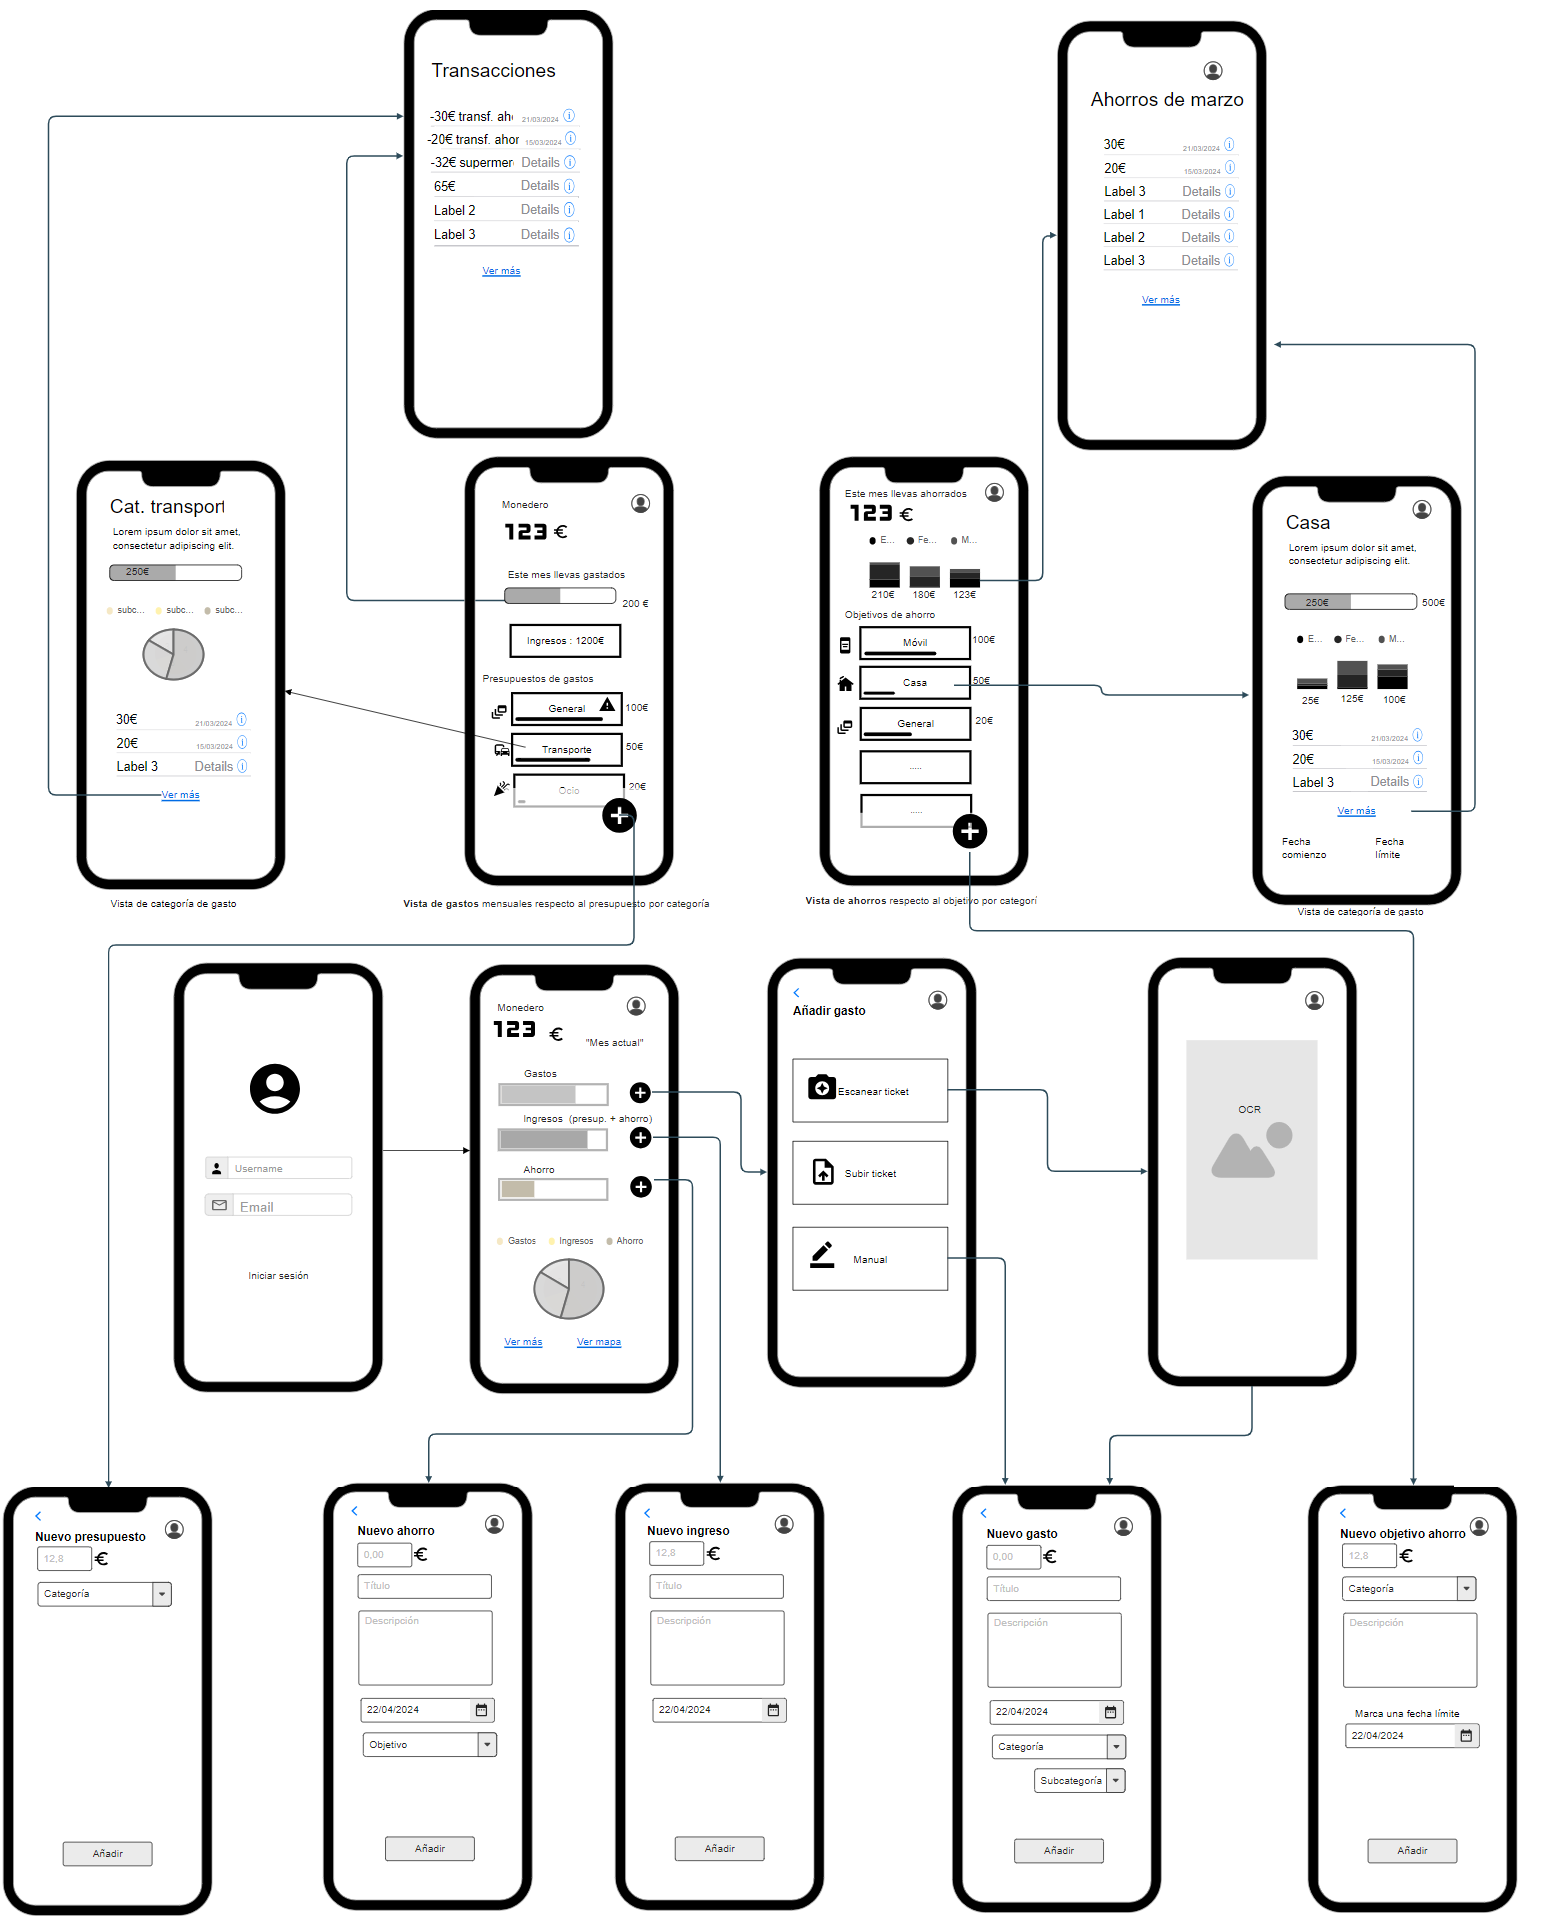
\includegraphics[width=\linewidth]{imagenes/wireframe.moqups.png}
    \caption{Wireframes de la interfaz de usuario en la aplicación}
    \label{fig:wireframes_vistas}
\end{figure}
